\documentclass[12pt]{article}
%\usepackage[utf8]{inputenc}
%\documentclass[UTF8]{ctexart}
%\usepackage[UTF8, heading = false, scheme = plain]{ctex}
\usepackage{geometry}
%geometry{a4paper,scale=0.9}
\geometry{a4paper,left=1cm,right=1cm,top=1cm,bottom=2cm}
\usepackage{amsfonts}
\usepackage{color}
\usepackage{url}
%\usepackage{biblatex}
\usepackage{amsmath}
\usepackage{amssymb}
\usepackage{latexsym}
\usepackage{cite}
%\addbibresource{ref.bib}
%\bibliography{ref.bib}
\usepackage{caption}
\usepackage{graphicx, subfig}
\usepackage{float}
%\usepackage[fontset=ubuntu]{ctex}
%\usepackage{fontspec}
\usepackage{xeCJK}
%\usepackage[colorlinks,
%anchorcolor=black,
%citecolor=black]{hyperref}
%\setmainfont{SimSun}
\usepackage[section]{placeins}
\usepackage{enumitem}
\usepackage{framed}
\usepackage[framemethod=TikZ]{mdframed}
\usepackage{indentfirst}
\usepackage{setspace}%使用间距宏包
\linespread{1.5}

\title{进程线程相关}
\author{leolinuxer}
%\date{June 2020}

\begin{document}
%\setlength{\parindent}{0pt}
\maketitle
\tableofcontents

\section{设置多少线程合适\cite{Multi_Thread_How_Many}}
\subsection{前言}
“不好了,线上服务器超时严重,请求非常慢,好像报连接数too many了,怎么办?“小伙伴们在反馈。一般我们的技术老大的处理方式,把连接数和线程池调大点,重启,再观察。

往往这个方式是应急措施,治标不治本,因为不知道问题的原因。而且大家会有个严重误区,以为线程池设置太小了,调大点请求就会快了。

今天就带着小伙伴们沟通一下,线程池的大小应该如何合理的设置其大小?

\subsection{问题}
如果有两个任务需要处理,一个任务A,一个任务B

方案一:一个线程执行任务A和B,A执行完后,执行B 方案二:两个线程A和B去执行任务A 和 B,同时进行

哪个方案会快点?应该很多人会回答,肯定是方案二啊,多线程并行去处理任务A和B,肯定快啊。是这样吗?回答这个问题之前,先带着大家去回顾梳理一下。

\subsection{线程执行}
线程的执行,是由CPU进行调度的,一个CPU在同一时刻只会执行一个线程,我们看上去的线程A 和 线程B并发执行。为了让用户感觉这些任务正在同时进行,操作系统利用了时间片轮转的方式,CPU给每个任务都服务一定的时间,然后把当前任务的状态保存下来,在加载下一任务的状态后,继续服务下一任务。任务的状态保存及再加载,这段过程就叫做\textbf{上下文切换}。

上下文切换过程是需要时间的;现在我们来看一下上面的问题,小伙伴们再看一下是哪个方案快呢?是不是有些小伙伴们会说方案一,因为不需要线程切换;方案二需要来回切换这两个线程,耗时会多点。

小伙伴们心中此时是不是会有疑惑,那为什么会有多线程?先不急,再往下看。

\subsection{为什么要多线程}
小伙伴想想在我们真实业务中,我们是什么流程?
\begin{figure}[H]
    \centering
    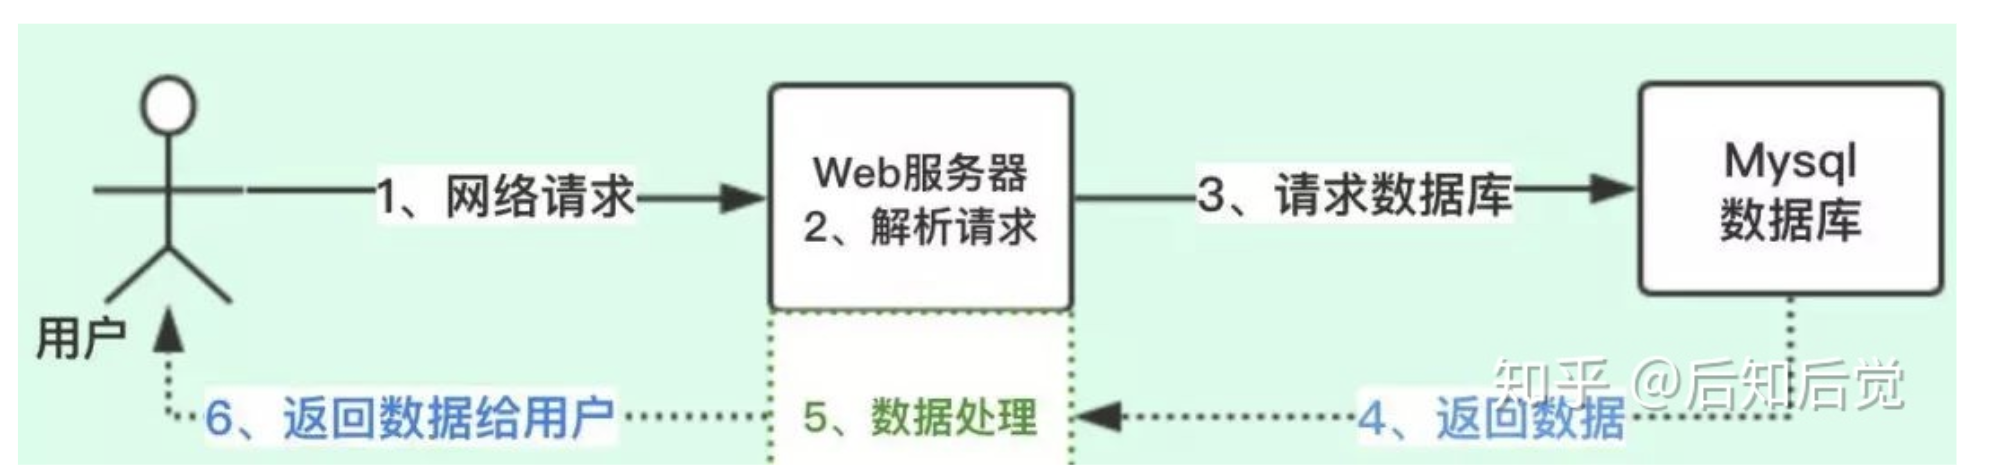
\includegraphics[width=1\textwidth]{fig/Multi_Thread_How_Many_1.png}
\end{figure}

上图的流程:
\begin{enumerate}
\setlength{\itemsep}{0pt}
\setlength{\parsep}{0pt}
\setlength{\parskip}{0pt}
    \item 先发起网络请求
    \item Web服务器解析请求
    \item 请求后端的数据库获取数据
    \item 获取数据后,进行处理
    \item 把处理结果放回给用户
\end{enumerate}

这个是我们处理业务的时候,常规的请求流程;我们看一下整个过程涉及到什么计算机处理。
\begin{itemize}
\setlength{\itemsep}{0pt}
\setlength{\parsep}{0pt}
\setlength{\parskip}{0pt}
    \item 网络请求----->网络IO
    \item 解析请求----->CPU
    \item 请求数据库----->网络IO
    \item MySQL查询数据----->磁盘IO
    \item MySQL返回数据----->网络IO
    \item 数据处理----->CPU
    \item 返回数据给用户----->网络IO
\end{itemize}

在真实业务中我们不单单会涉及CPU计算,还有网络IO和磁盘IO处理,这些处理是非常耗时的。如果一个线程整个流程是上图的流程,真正涉及到CPU的只有2个节点,其他的节点都是IO处理,那么线程在做IO处理的时候,CPU就空闲出来了,CPU的利用率就不高。

小伙伴们现在知道多线程的用处了吧,对,就是\textbf{为了提升CPU利用率}。

\subsection{提升QPS/TPS}
衡量系统性能如何,主要指标系统的(QPS/TPS)
\begin{itemize}
\setlength{\itemsep}{0pt}
\setlength{\parsep}{0pt}
\setlength{\parskip}{0pt}
    \item QPS/TPS:每秒能够处理请求/事务的数量
    \item 并发数:系统同时处理的请求/事务的数量
    \item 响应时间:就是平均处理一个请求/事务需要时长
\end{itemize}

QPS/TPS = 并发数/响应时间

上面公式代表\textbf{并发数越大,QPS就越大};所以很多人就会以为调大线程池,并发数就会大,也会提升QPS,所以才会出现一开始前言所说的,大多数人的误区。

其实\textbf{QPS还跟响应时间成反比,响应时间越大,QPS就会越小}。

虽然并发数调大了,就会提升QPS,但线程数也会影响响应时间,因为上面我们也提到了上下文切换的问题,那怎么设置线程数的呢?

\subsection{如何设置线程数}
那我们如何分配线程?我们提供一个公式:

最佳线程数目 = ((线程等待时间+线程CPU时间)/线程CPU时间 )* CPU数目

备注这个公式也是前辈们分享的,当然之前看了淘宝前台系统优化实践的文章,和上面的公式很类似,不过在CPU数目那边,他们更细化了,上面的公式只是参考。不过不管什么公式,最终还是在生产环境中运行后,再优化调整。

我们继续上面的任务,我们的服务器CPU核数为4核,一个任务线程cpu耗时为20ms,线程等待(网络IO、磁盘IO)耗时80ms,那最佳线程数目:( 80 + 20 )/20 * 4 = 20。也就是设置20个线程数最佳。

从这个公式上面我们就得出,\textbf{线程的等待时间越大,线程数就要设置越大},这个正好符合我们上面的分析,可提升CPU利用率。那从另一个角度上面说,线程数设置多大,是根据我们自身的业务的,需要自己去压力测试,设置一个合理的数值。

\subsection{基础常规标准}
那我们小伙伴们会问,因为很多业务集中到一个线程池中,不像上面的案例比较简单,事实上业务太多,怎么设置呢?这个就是要去压力测试去调整。不过我们的前辈已经帮我们总结了一个基础的值(最终还是要看运行情况自行调整):

1、CPU密集型:操作内存处理的业务,一般线程数设置为:CPU核数 + 1 或者 CPU核数*2。核数为4的话,一般设置 5 或 8;

2、IO密集型:文件操作,网络操作,数据库操作,一般线程设置为:cpu核数 / (1-0.9),核数为4的话,一般设置 40;



%\printbibliography
\bibliography{../ref}
\bibliographystyle{IEEEtran}
\end{document}